\section{Verdeckung durch Pointcloud Projektion} \label{sec:pc-projection}

Die erste und weniger aufwändige Idee eine Überlagerung in Augmented Reality zu realisieren, ist die Überführung der Pointcloud in eine Depthmap, die wiederum in den Renderingprozess mit eingebracht wird. Das Verfahren von \citet{kanbara2000stereoscopic} verfolgt einen ähnlichen Weg mit einer Stereokamera und einer video see-through Displaytechnologie in Form eines Head-Mounted Display. Wie in Abbildung \ref{fig:stereo-depth-map} zu erkennen, bestimmen sie mit Hilfe der Stereokamera Tiefeninformationen, die das gerenderte virtuelle Objekt an den Positionen ausspart, an denen Tiefeninformationen im Vordergrund vorliegen. Aufgrund von weiteren Forschungsergebnissen aus dem Bereich des Stereomatchings, erreichen sie bessere Ergebnisse als \citet{wloka1995resolving}, die das Vorgehen als Erste vorgestellt haben.

\begin{figure}[h]
  \centering
	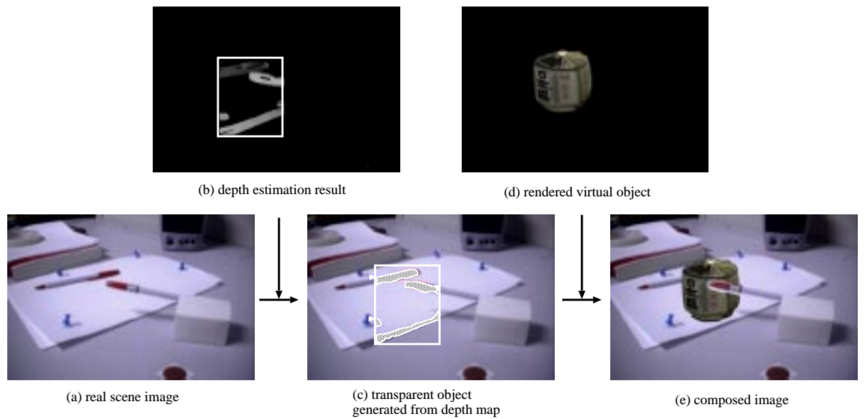
\includegraphics[width=1.0\textwidth]{content/images/methods/stereo-depth-map.png} 
  \caption{Visualisierung der Methode zur Vedeckung durch Depth Maps. Übernommen von \citet{kanbara2000stereoscopic}}
  \label{fig:stereo-depth-map}
\end{figure}

Anders als im Verfahren von \citet{kanbara2000stereoscopic} wird hier eine Depthmap anhand der vorhandenen Pointcloud aus dem Infrarotsensor von Project Tango gewonnen. Dadurch, dass die intrinsischen Kameraeigenschaften der Farbkamera zur Verfügung stehen, welche auch die Aufnahmequelle der Infrarotpunkte ist, kann ein Punkt \(P = [X, Y, Z]\) der Pointcloud mit der Gleichung \ref{eq:projection} auf die Bildebene überführt werden. Hier stehen die Variablen \(f_{x/y}\) für die Brennweite und \(c_{x/y}\) für den Bildmittelpunkt auf der Bildebene. \citep{Tango90:online}

\begin{equation}\label{eq:projection}
x = \frac{X* f_x * \frac{r_d}{r_u}}{Z}  + c_x
\qquad
y = \frac{Y* f_y * \frac{r_d}{r_u}}{Z}  + c_y
\end{equation}

Da die Linsen einer Kamera nie perfekte Brechungseigenschaften besitzen, muss an dieser Stelle auch die Verzerrung der Linse mit berücksichtigt werden. In den Gleichungen aus \ref{eq:projection} ist diese Verzerrung in den Parametern \(\frac{r_d}{r_u}\) enthalten. Zur Kalibrierung der Linse wird bei Project Tango für die normale Farbkamera und somit auch für die Aufnahme der Infrarotpunkte die Technik von \citet{tsai1987versatile} verwendet  \citep{Tango90:online}. Das hier beschriebene Verzerrungsmodell basiert dabei auf den drei Parametern \(k_{1} \downarrow  k_{3}\), welche die radiale Verzerrung ausgehend vom Linsenmittelpunkt modellieren kann. Hierzu wird für jeden Punkt, wie in Gleichung \ref{eq:distortion} gezeigt, die radiale Distanz \(r_u\) zum Linsenmittelpunkt und die durch die Linseneigenschaft verzerrte radiale Distanz \(r_d\) ermittelt. Dieses Verhältnis streckt oder staucht die Position radial auf der Bildebene.


\begin{equation} \label{eq:distortion}
r_u = \sqrt{\frac{X^2 + Y^2}{ Z^2}} 
\qquad
r_d = r_u + k_1 * r_u^3 + k_2 * r_u^5 + k_3 * r_u^7
\end{equation}

An dieser berechneten Position auf der Bildebene bzw. Depthmap wird nun ein Punkt mit einem Graustufenwert, entsprechend der Entfernung \(|\overrightarrow{PO_{cam}}|\) vom Punkt \(P\) zum Kameraursprung \(O_{cam}\) gezeichnet. Der Farbwert richtet sich dabei nach der Konvention des Renderingframeworks und den Informationen über die vordere und hintere Clippingebene.

Die Auflösung des Tiefensensors der Project Tango Hardware ist mit \(320 \times 180\) Pixeln gegenüber der Auflösung der Farbkamera mit \(1280 \times 720\) vier mal kleiner. Zusätzlich ist die Dichte der Pointcloud zum eigentlichen Sensor geringer als ihre eigene Auflösung. So würde man bei einer Auflösung von \(320 \times 180 = 57600\) Tiefenpunkte bei idealen Verhältnissen erwarten. Project Tango liefert jedoch unter guten Bedingungen durchschnittlich \(17000\) Tiefenpunkte. Aufgrund der kleineren Auflösung und der geringeren Informationsdichte werden die gezeichneten Punkte auf der Depthmap hier mit einem Radius von 4 Bildpunkten gezeichnet. 

Nachdem die Depthmap generiert wurde, kann zum Ausschluss der Pixel der virtuellen Objekte, welches sich hinter einem realen Objekt befinden, der Z-Buffer Algorithmus aus Kapitel \ref{sec:z-buffer} wie von \citet{wloka1995resolving} beschrieben, angewendet werden. Hierzu wird vor dem virtuellen Rendering der Z-Buffer mit den generierten Informationen aus der Depthmap gefüllt. Pixel der virtuellen Objekte werden somit nicht gerendert, wenn an dieser Position eine geringere Distanz zu realen Objekten in den Tiefeninformationen vorliegen. 


